\documentclass[aspectratio=169,10pt]{beamer}

% =========================================================
% PACKAGES
% =========================================================
\usepackage[T1]{fontenc}
\usepackage{lmodern}
\usepackage{amsmath,amssymb}
\usepackage{booktabs}
\usepackage{array}
\usepackage{tikz}
\usepackage{ragged2e}
\usetikzlibrary{arrows.meta,positioning,calc}

% =========================================================
% METROPOLIS
% =========================================================
\usetheme[numbering=fraction]{metropolis}
\setbeamertemplate{navigation symbols}{}

% =========================================================
% COLORS
% =========================================================
\definecolor{Navy}{RGB}{25,55,85}
\definecolor{Blue}{RGB}{40,105,175}
\definecolor{Orange}{RGB}{225,125,20}
\definecolor{Red}{RGB}{190,45,45}
\definecolor{GrayPath}{RGB}{185,185,185}
\definecolor{LightBlue}{RGB}{235,245,255}
\definecolor{LightOrange}{RGB}{255,244,225}
\definecolor{LightRed}{RGB}{255,235,235}

\setbeamercolor{frametitle}{fg=Navy,bg=white}
\setbeamersize{text margin left=0.70cm,text margin right=0.70cm}
\setbeamerfont{frametitle}{size=\Large,series=\bfseries}
\setbeamercolor{author in head/foot}{fg=Navy,bg=white}
\setbeamertemplate{frametitle}{%
  \nointerlineskip
  \begin{beamercolorbox}[wd=\paperwidth,ht=1.02cm,dp=0.20cm,leftskip=0.70cm,rightskip=0.70cm]{frametitle}%
    \usebeamerfont{frametitle}\insertframetitle
  \end{beamercolorbox}%
  \nointerlineskip
  \begin{beamercolorbox}[wd=\paperwidth,ht=1.25pt,dp=0pt]{normal text}%
    \hspace*{0.70cm}\color{Orange}\rule{\dimexpr\paperwidth-1.40cm\relax}{1.25pt}%
  \end{beamercolorbox}%
}
\setbeamercolor{normal text}{fg=black,bg=white}
\hbadness=10000
\vbadness=10000

% =========================================================
% FOOTER
% =========================================================
\setbeamertemplate{footline}{%
  \leavevmode
  \hbox to \paperwidth{%
    \begin{beamercolorbox}[wd=.40\paperwidth,ht=2.8ex,dp=1.0ex,leftskip=0.8em]{author in head/foot}
      \scriptsize\textbf{Industrial Management | Unit--V}
    \end{beamercolorbox}%
    \begin{beamercolorbox}[wd=.45\paperwidth,ht=2.8ex,dp=1.0ex,center]{author in head/foot}
      \scriptsize Gajavada Sanjeevkumar
    \end{beamercolorbox}%
    \begin{beamercolorbox}[wd=.15\paperwidth,ht=2.8ex,dp=1.0ex,rightskip=0.8em]{author in head/foot}
      \hfill\scriptsize\insertframenumber
    \end{beamercolorbox}%
  }
  \vskip0pt\hbox to \paperwidth{\color{Navy!20}\rule{\paperwidth}{0.5pt}}
}

% =========================================================
% HIGHLIGHT COMMANDS
% =========================================================
\newcommand{\maxmark}[1]{\textcolor{Blue}{\textbf{MAX = #1}}}
\newcommand{\minmark}[1]{\textcolor{Orange}{\textbf{MIN = #1}}}
\newcommand{\answer}[1]{\textbf{Answer: #1}}
\newcommand{\criticaltext}[1]{\begin{center}\parbox{0.78\textwidth}{\centering\textcolor{Red}{\textbf{#1}}}\end{center}}
\newcommand{\teachstep}[1]{\par\medskip\noindent\textbf{#1}\par\smallskip}

% =========================================================
% NETWORK STYLES
% Selected path = bright orange highlight.
% All other paths = light gray, never dark-filled.
% =========================================================
\tikzset{
  event/.style={circle,draw=Navy,thick,minimum size=7.5mm,font=\bfseries},
  basepath/.style={->,>=Stealth,thin,draw=GrayPath,line width=0.75pt},
  highlightpath/.style={->,>=Stealth,very thick,draw=Orange,line width=2.6pt},
  activitylabel/.style={font=\scriptsize},
  act/.style={draw=Navy,rounded corners,fill=white,minimum width=0.95cm,minimum height=0.55cm,font=\scriptsize,align=center},
  actpath/.style={->,>=Stealth,thin,draw=GrayPath,line width=0.75pt,shorten >=0.43cm,shorten <=0.43cm},
  acthighlight/.style={->,>=Stealth,very thick,draw=Orange,line width=2.6pt,shorten >=0.43cm,shorten <=0.43cm}
}

% =========================================================
% TITLE INFORMATION
% =========================================================
\title{Industrial Management}
\subtitle{Unit-V: Job Evaluation and Project Management (PERT\&CPM)}

\author{
    \textbf{Gajavada Sanjeevkumar}
}
\date{}

\begin{document}

\begin{frame}[plain]
\vspace{1.35cm}

{\usebeamerfont{title}\color{black}\bfseries\LARGE Industrial Management\par}

\vspace{0.32cm}

{\large Unit--V: Job Evaluation and Project Management (PERT\&CPM)\par}

\vspace{0.28cm}

{\color{Orange}\rule{\textwidth}{1.4pt}\par}

\vfill

{\large\textbf{Gajavada Sanjeevkumar}\par}

\vspace{0.7cm}

\end{frame}

% =========================================================
% SYLLABUS
% =========================================================


% =========================================================
% JOB EVALUATION
% =========================================================
\section{Job Evaluation}

\begin{frame}{Job Evaluation: What?}
\begin{block}{Meaning}
Job evaluation is a systematic process of determining the relative worth of jobs within an organization.
\end{block}
\begin{itemize}
  \item It evaluates the \textbf{job}, not the individual employee occupying the job.
  \item Jobs are compared using consistent, defined criteria.
  \item The result supports a rational internal hierarchy of jobs and wage/salary relationships.
\end{itemize}
\end{frame}

\begin{frame}{Job Evaluation: Why Is It Needed?}
\begin{itemize}
  \item Different jobs require different levels of skill, responsibility, effort and working conditions.
  \item Without systematic comparison, job relationships may become inconsistent.
  \item It provides a common basis for discussing relative job worth.
  \item It helps management establish logical job grades and relationships.
\end{itemize}
\end{frame}

\begin{frame}{Job Evaluation: Where and When?}
\textbf{Where?}
\begin{itemize}
  \item Organizations with several jobs having different duties and responsibility levels.
\end{itemize}
\textbf{When?}
\begin{itemize}
  \item Designing or reviewing job grades.
  \item Designing or reviewing wage structures.
  \item Reviewing internal job relationships.
  \item Comparing many jobs consistently.
\end{itemize}
\vspace{0.15cm}
\textit{Job evaluation does not replace individual performance appraisal.}
\end{frame}

\begin{frame}{Job Evaluation: Basic Logic}
\centering
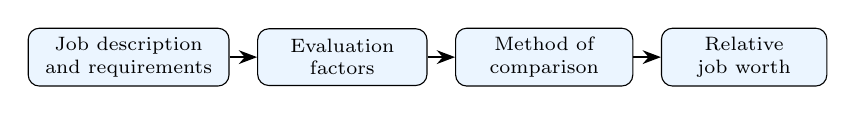
\begin{tikzpicture}[node distance=0.35cm]
\node[draw,rounded corners,fill=LightBlue,minimum width=2.55cm,minimum height=0.72cm,align=center,font=\scriptsize] (a) {Job description\\and requirements};
\node[draw,rounded corners,fill=LightBlue,minimum width=2.15cm,minimum height=0.72cm,align=center,font=\scriptsize,right=of a] (b) {Evaluation\\factors};
\node[draw,rounded corners,fill=LightBlue,minimum width=2.25cm,minimum height=0.72cm,align=center,font=\scriptsize,right=of b] (c) {Method of\\comparison};
\node[draw,rounded corners,fill=LightBlue,minimum width=2.10cm,minimum height=0.72cm,align=center,font=\scriptsize,right=of c] (d) {Relative\\job worth};
\draw[->,>=Stealth,thick](a.east)--(b.west);
\draw[->,>=Stealth,thick](b.east)--(c.west);
\draw[->,>=Stealth,thick](c.east)--(d.west);
\end{tikzpicture}
\vspace{0.35cm}
\begin{itemize}
  \item Describe the job and its requirements.
  \item Identify the factors used for comparison.
  \item Apply the selected evaluation method consistently.
  \item Obtain the relative worth of the job.
\end{itemize}
\end{frame}

\begin{frame}{Methods of Job Evaluation}
\begin{enumerate}
  \item Simple routing objective systems
  \item Classification method
  \item Factor comparison method
  \item Point method
\end{enumerate}
\vspace{0.25cm}
\begin{block}{Common purpose}
All four approaches seek a systematic basis for determining the relative worth of jobs.
\end{block}
\end{frame}

% Simple routing objective systems
\begin{frame}{Simple Routing Objective Systems: What?}
\begin{itemize}
  \item The syllabus emphasizes a simple, systematic and objective route for comparing jobs.
  \item A defined set of job-related criteria is used rather than personal preference.
  \item The evaluation follows a consistent sequence so comparable jobs are treated similarly.
\end{itemize}
\end{frame}

\begin{frame}{Simple Routing Objective Systems: How?}
\begin{enumerate}
  \item Collect job information.
  \item Identify criteria on which jobs are compared.
  \item Apply the same criteria to each job.
  \item Record the comparison systematically.
  \item Obtain the relative position/value of the jobs.
\end{enumerate}
\vspace{0.25cm}
\boxed{\text{Objective comparison}\;\rightarrow\;\text{consistent criteria}\;\rightarrow\;\text{repeatable result}}
\end{frame}

\begin{frame}{Simple Routing Objective Systems: Interpretation}
\begin{itemize}
  \item \textbf{What?} A simple structured route for job comparison.
  \item \textbf{Why?} To reduce arbitrary or inconsistent comparisons.
  \item \textbf{How?} Use the same defined criteria and sequence for comparable jobs.
  \item \textbf{Limitation?} Greater simplicity can reduce the depth and precision of the evaluation.
\end{itemize}
\end{frame}

% Classification
\begin{frame}{Classification Method: What?}
\begin{block}{Idea}
Jobs are placed into predefined classes or grades.
\end{block}
\begin{itemize}
  \item Each grade has a general description of duties, skill and responsibility.
  \item The job is compared with the grade descriptions.
  \item The job is assigned to the most appropriate class.
\end{itemize}
\end{frame}

\begin{frame}{Classification Method: Why and When?}
\begin{itemize}
  \item \textbf{Why:} relatively simple way to group many jobs.
  \item \textbf{When:} useful when clear grade descriptions can be defined.
  \item Easier to administer than a highly detailed numerical system.
  \item May be less precise when a job falls between class descriptions.
\end{itemize}
\end{frame}

\begin{frame}{Classification Method: Procedure}
\begin{enumerate}
  \item Define job classes/grades.
  \item Write a clear description for each class.
  \item Study the job being evaluated.
  \item Compare duties and requirements with class descriptions.
  \item Assign the job to the best-fitting class.
  \item Review consistency with other evaluated jobs.
\end{enumerate}
\end{frame}

\begin{frame}{Classification Method: Diagram}
\centering
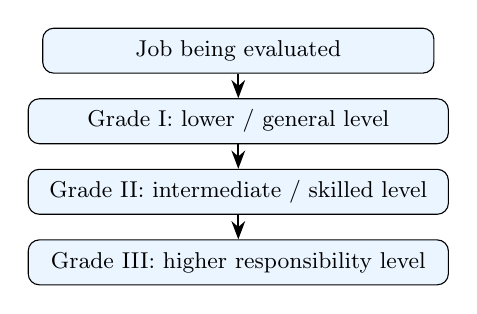
\begin{tikzpicture}[node distance=0.34cm,scale=0.92,transform shape]
\node[draw,rounded corners,fill=LightBlue,minimum width=5.4cm,minimum height=0.62cm,align=center,font=\small] (j) {Job being evaluated};
\node[draw,rounded corners,fill=LightBlue,minimum width=5.8cm,minimum height=0.62cm,align=center,font=\small,below=of j] (g1) {Grade I: lower / general level};
\node[draw,rounded corners,fill=LightBlue,minimum width=5.8cm,minimum height=0.62cm,align=center,font=\small,below=of g1] (g2) {Grade II: intermediate / skilled level};
\node[draw,rounded corners,fill=LightBlue,minimum width=5.8cm,minimum height=0.62cm,align=center,font=\small,below=of g2] (g3) {Grade III: higher responsibility level};
\draw[->,>=Stealth,thick](j.south)--(g1.north);
\draw[->,>=Stealth,thick](g1.south)--(g2.north);
\draw[->,>=Stealth,thick](g2.south)--(g3.north);
\end{tikzpicture}
\vspace{0.35cm}
\begin{beamercolorbox}[wd=0.82\textwidth,sep=0.18cm,center]{normal text}
\small The job is placed in the grade whose description most closely matches its duties and requirements.
\end{beamercolorbox}
\end{frame}

\begin{frame}{Classification Method: Simple Example}
\centering
\begin{tabular}{c|l|l}
\toprule
Grade & General description & Example placement\\
\midrule
I & Routine/general duties & Routine assistant job\\
II & Skilled/intermediate duties & Skilled technician job\\
III & Higher responsibility & Supervisory job\\
\bottomrule
\end{tabular}
\vspace{0.3cm}

If a job's duties match Grade II most closely, it is classified as Grade II.
\end{frame}

% Factor comparison
\begin{frame}{Factor Comparison Method: What?}
\begin{itemize}
  \item Jobs are compared \textbf{factor by factor}.
  \item Benchmark jobs are selected first.
  \item Compensable factors represent important characteristics of jobs.
  \item Each job receives a relative value for each factor; the factor values are then combined.
\end{itemize}
\end{frame}

\begin{frame}{Factor Comparison: Typical Factors}
Typical factors used to explain the method include:
\begin{itemize}
  \item Skill
  \item Responsibility
  \item Effort
  \item Working conditions
\end{itemize}
\vspace{0.25cm}
\textbf{Interpretation:} a job may be higher in one factor and lower in another; factor comparison makes those differences explicit.
\end{frame}

\begin{frame}{Factor Comparison: Procedure}
\begin{enumerate}
  \item Select representative benchmark jobs.
  \item Select factors used for comparison.
  \item Rank benchmark jobs factor by factor.
  \item Assign relative/monetary values to the factors.
  \item Compare other jobs with benchmark jobs factor by factor.
  \item Add factor values to obtain the job's total relative value.
\end{enumerate}
\end{frame}

\begin{frame}{Factor Comparison: Mathematical Interpretation}
For factors $1,\ldots,k$:
\[
\boxed{J=\sum_{i=1}^{k}v_i}
\]
where $v_i$ is the value assigned to factor $i$ for the job.

\vspace{0.2cm}
The important examination step is to perform the comparison \textbf{factor by factor before summing}.
\end{frame}

\begin{frame}{Factor Comparison: Worked Numerical Problem}
\small
\textbf{Problem.} Three jobs are evaluated using four factors. Calculate the total relative value of each job.
\vspace{0.18cm}
\begin{center}
\begin{tabular}{c|rrrr|r}
\toprule
Job & Skill & Responsibility & Effort & Conditions & Total\\
\midrule
X & 40 & 35 & 25 & 10 & --\\
Y & 35 & 40 & 30 & 15 & --\\
Z & 45 & 30 & 25 & 10 & --\\
\bottomrule
\end{tabular}
\end{center}
\vspace{0.15cm}
\textbf{Required:} add the four factor values for each job and compare the totals.
\end{frame}

\begin{frame}{Factor Comparison: Job X}
\small
\par\textbf{Step 1:} Add the four factor values for Job X.
\[
J_X=40+35+25+10
\]
\pause
\par\textbf{Step 2:} Combine the first two factors.
\[
J_X=75+25+10
\]
\pause
\par\textbf{Step 3:} Continue the addition.
\[
J_X=100+10
\]
\pause
\par\textbf{Step 4:} Total relative value.
\[
\boxed{J_X=110}
\]
\end{frame}

\begin{frame}{Factor Comparison: Jobs Y and Z}
\small
\textbf{Job Y -- Step 1}
\[
J_Y=35+40+30+15
\]
\pause
\textbf{Job Y -- Step 2}
\[
J_Y=75+30+15=105+15=\boxed{120}
\]
\pause
\textbf{Job Z -- Step 1}
\[
J_Z=45+30+25+10
\]
\pause
\textbf{Job Z -- Step 2}
\[
J_Z=75+25+10=100+10=\boxed{110}
\]
\end{frame}

\begin{frame}{Factor Comparison: Interpretation}
\small
\begin{center}
\begin{tabular}{c|c}
\toprule Job & Total relative value\\\midrule
X&110\\Y&120\\Z&110\\\bottomrule
\end{tabular}
\end{center}
\vspace{0.18cm}
\par\textbf{Step 1:} Compare the totals.
\[
120>110=110
\]
\pause
\par\textbf{Step 2:} Interpret the comparison.
Job Y has the highest total in this illustration; Jobs X and Z have equal totals although their factor profiles differ.
\end{frame}

\begin{frame}{Point Method: What?}
\begin{itemize}
  \item Assign numerical points to defined compensable factors and their degrees.
  \item Evaluate the job factor by factor.
  \item Sum the selected points to obtain a total job score.
  \item Higher total points indicate higher relative job value within the evaluation system.
\end{itemize}
\end{frame}

\begin{frame}{Point Method: Why?}
\begin{itemize}
  \item Converts qualitative job differences into a numerical score.
  \item Provides a systematic basis for comparing many jobs.
  \item Makes the selected factor and degree visible.
  \item Allows jobs to be arranged in relative order using total scores.
\end{itemize}
\end{frame}

\begin{frame}{Point Method: Procedure}
\begin{enumerate}
  \item Select compensable factors.
  \item Define degrees/levels for each factor.
  \item Assign points to the degrees.
  \item Examine the job and select the appropriate degree for each factor.
  \item Add the selected points.
  \item Compare the total score with other jobs.
\end{enumerate}
\end{frame}

\begin{frame}{Point Method: Structure}
\centering
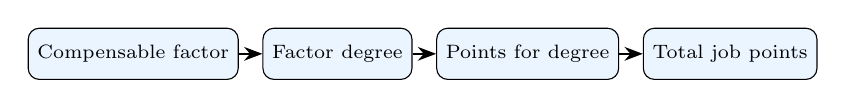
\begin{tikzpicture}[node distance=0.3cm]
\node[draw,rounded corners,fill=LightBlue,minimum width=1.95cm,minimum height=0.65cm,align=center,font=\scriptsize] (a) {Compensable factor};
\node[draw,rounded corners,fill=LightBlue,minimum width=1.75cm,minimum height=0.65cm,align=center,font=\scriptsize,right=of a] (b) {Factor degree};
\node[draw,rounded corners,fill=LightBlue,minimum width=1.95cm,minimum height=0.65cm,align=center,font=\scriptsize,right=of b] (c) {Points for degree};
\node[draw,rounded corners,fill=LightBlue,minimum width=1.95cm,minimum height=0.65cm,align=center,font=\scriptsize,right=of c] (d) {Total job points};
\draw[->,>=Stealth,thick](a.east)--(b.west);
\draw[->,>=Stealth,thick](b.east)--(c.west);
\draw[->,>=Stealth,thick](c.east)--(d.west);
\end{tikzpicture}
\vspace{0.35cm}
\begin{itemize}
  \item Select a compensable factor.
  \item Determine the appropriate degree and its assigned points.
  \item Add the selected points for all factors to obtain the total job score.
\end{itemize}
\[J=\sum_i p_i\]
where $p_i$ is the selected point value for factor $i$.
\end{frame}

\begin{frame}{Point Method: Worked Numerical Problem}
\centering\small
\begin{tabular}{l|c|r}
\toprule
Factor & Selected degree & Points\\
\midrule
Skill & III & 60\\
Responsibility & IV & 50\\
Effort & III & 30\\
Working conditions & II & 20\\
Education & II & 25\\
\bottomrule
\end{tabular}
\vspace{0.2cm}
Determine the total job points.
\end{frame}

\begin{frame}{Point Method: Step 1 -- Select the Points}
The job is evaluated factor by factor.
\pause
Skill, degree III:
\[p_1=60\]
\pause
Responsibility, degree IV:
\[p_2=50\]
\pause
Effort, degree III:
\[p_3=30\]
\end{frame}

\begin{frame}{Point Method: Step 2 -- Remaining Factors}
Working conditions, degree II:
\pause
\[p_4=20\]
\pause
Education, degree II:
\[p_5=25\]
\pause
The selected points are therefore:
\[60,\;50,\;30,\;20,\;25.\]
\end{frame}

\begin{frame}{Point Method: Step 3 -- Total Job Points}
\[J=60+50+30+20+25\]
\pause
\[J=110+30+20+25\]
\pause
\[J=140+20+25\]
\pause
\[J=160+25\]
\pause
\[\boxed{J=185\text{ points}}\]
\end{frame}

\begin{frame}{Benefits of Job Evaluation}
\begin{itemize}
  \item Systematic basis for comparing jobs.
  \item Helps establish internal consistency in job relationships.
  \item Makes the basis of job comparisons clearer.
  \item Supports structured job grades and wage/salary relationships.
  \item Helps management review whether jobs have similar relative requirements.
\end{itemize}
\end{frame}

\begin{frame}{Limitations of Job Evaluation}
\begin{itemize}
  \item Selection and weighting of factors involve judgment.
  \item Job content may change, requiring reevaluation.
  \item Detailed systems can require time and administrative effort.
  \item Job evaluation does not measure individual employee performance.
  \item The result is a relative evaluation within the organization's chosen framework.
\end{itemize}
\end{frame}

\begin{frame}{Job Evaluation: Comparison of Listed Methods}
\centering
\small
\begin{tabular}{l|l|l}
\toprule
Method & Main basis & Basic output\\
\midrule
Simple routing objective systems & Defined objective route/criteria & Relative comparison\\
Classification & Predefined grades/classes & Grade assigned\\
Factor comparison & Factor-by-factor comparison & Combined factor value\\
Point method & Points for factor degrees & Total point score\\
\bottomrule
\end{tabular}
\end{frame}

% =========================================================
% PROJECT MANAGEMENT / NETWORK ANALYSIS
% =========================================================
\section{Project Management and Network Analysis}

\begin{frame}{Project Management (PERT/CPM)}
\begin{block}{Project}
A project is a collection of interrelated activities undertaken to achieve a defined objective.
\end{block}
\begin{itemize}
  \item Activities have precedence relationships.
  \item Some activities cannot start until others are completed.
  \item PERT/CPM provides a network-based way to analyse project time and, within this syllabus, project cost/crashing.
\end{itemize}
\end{frame}

\begin{frame}{Network Analysis: Why?}
\begin{itemize}
  \item A project may contain many activities with dependencies.
  \item A simple activity list does not show the complete logical sequence.
  \item A network shows precedence relationships.
  \item Network analysis allows systematic calculation of project duration.
  \item It provides the basis for identifying the critical path.
\end{itemize}
\end{frame}

\begin{frame}{Network Analysis: Basic Terms}
\begin{description}
\item[Activity] A task that consumes time and usually resources.
\item[Event] A point marking the start or completion of activities in an activity-on-arrow representation.
\item[Predecessor] An activity that must be completed before another can begin.
\item[Successor] An activity that follows another activity.
\item[Path] A connected sequence of activities from project start to finish.
\end{description}
\end{frame}

\begin{frame}{Network Representation}
\centering
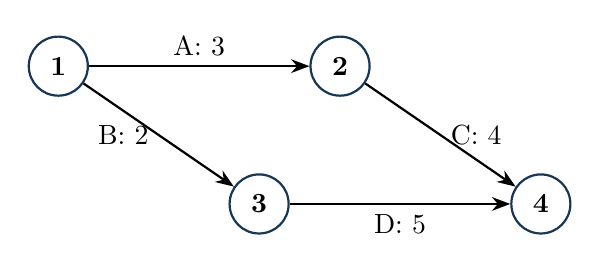
\begin{tikzpicture}[node distance=2.8cm]
\node[event](a){1};
\node[event,right=of a](b){2};
\node[event,below right=1.2cm and 2.0cm of a](c){3};
\node[event,right=of c](d){4};
\draw[->,>=Stealth,thick](a)--node[above]{A: 3}(b);
\draw[->,>=Stealth,thick](a)--node[left]{B: 2}(c);
\draw[->,>=Stealth,thick](b)--node[right]{C: 4}(d);
\draw[->,>=Stealth,thick](c)--node[below]{D: 5}(d);
\end{tikzpicture}
\vspace{0.3cm}

Arrows represent activities; nodes represent events.
\end{frame}

\begin{frame}{Network Construction: How?}
\begin{enumerate}
  \item List all activities.
  \item Determine immediate predecessors.
  \item Draw the network in precedence order.
  \item Assign durations.
  \item Verify all precedence relationships.
  \item Perform time calculations.
  \item Identify the critical path.
\end{enumerate}
\end{frame}

\begin{frame}{Simple Network: Activity Table}
\centering
\begin{tabular}{c|c|c}
\toprule
Activity & Duration & Predecessor\\
\midrule
A & 3 & --\\
B & 4 & A\\
C & 2 & A\\
D & 5 & B, C\\
\bottomrule
\end{tabular}
\vspace{0.35cm}

\textbf{Important:} D can start only after both B and C are complete.
\end{frame}

\begin{frame}{Network Construction: Complete Worked Network}
\centering
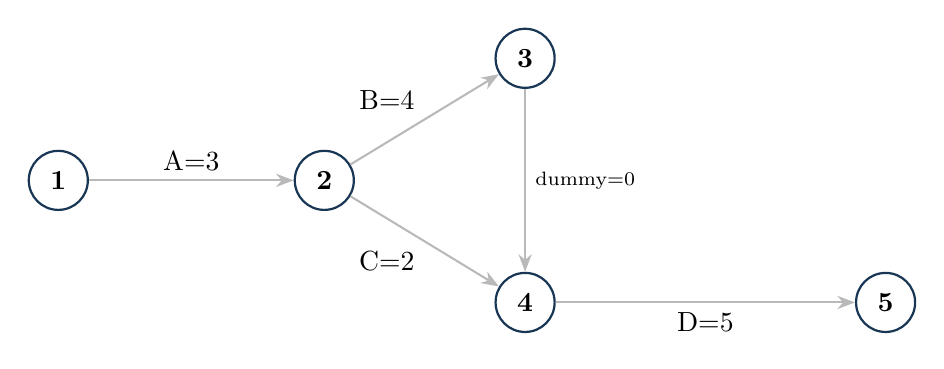
\begin{tikzpicture}[node distance=2.6cm]
\node[event](1){1};
\node[event,right=of 1](2){2};
\node[event,above right=1.0cm and 2.0cm of 2](3){3};
\node[event,below right=1.0cm and 2.0cm of 2](4){4};
\node[event,right=3.8cm of 4](5){5};
\draw[basepath](1)--node[above]{A=3}(2);
\draw[basepath](2)--node[above left]{B=4}(3);
\draw[basepath](2)--node[below left]{C=2}(4);
\draw[basepath](3)--node[right,activitylabel]{dummy=0}(4);
\draw[basepath](4)--node[below]{D=5}(5);
\end{tikzpicture}
\vspace{0.2cm}

The two complete paths are formed through B and C, with a zero-duration dummy activity enforcing the precedence relationship before D.
\end{frame}

\begin{frame}{Why is the Dummy Activity $3\rightarrow4$ Needed?}
\small
\begin{block}{Required precedence}
Activity $D$ must start only after both $B$ and $C$ are completed.
\end{block}

\begin{columns}[T,totalwidth=\textwidth]
\column{0.48\textwidth}
\textbf{With the dummy:}
\[
B:~2\rightarrow3,\qquad dummy:~3\rightarrow4
\]
Therefore event 4 occurs only after both $B$ and $C$ are complete:
\[
\boxed{D\text{ requires }B\text{ and }C}
\]
The dummy has zero duration and represents only a logical precedence relationship.

\column{0.48\textwidth}
\textbf{If we draw $3\rightarrow5$ directly:}
\[
B:~2\rightarrow3\rightarrow5
\]
while $D$ still starts from event 4 after $C$. Hence $D$ would no longer depend on $B$:
\[
\boxed{D\text{ would require only }C}
\]
So the direct $3\rightarrow5$ connection changes the project logic.
\end{columns}

\vspace{0.18cm}
\centering
\textbf{Conclusion:} The dummy $3\rightarrow4$ is necessary to represent the stated precedence correctly.
\end{frame}

% =========================================================
% PATH HIGHLIGHTING -- EACH PATH ONCE
% =========================================================
\begin{frame}{Path 1 Highlighted: $A\rightarrow B\rightarrow D$}
\centering
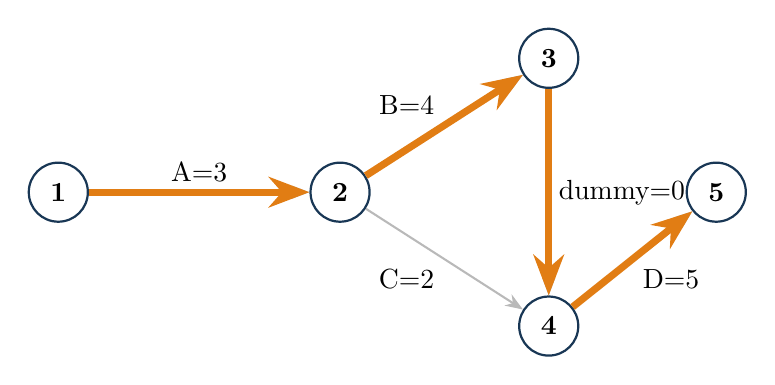
\begin{tikzpicture}[node distance=2.8cm]
\node[event](1){1};\node[event,right=of 1](2){2};\node[event,above right=1.15cm and 2.1cm of 2](3){3};\node[event,below right=1.15cm and 2.1cm of 2](4){4};\node[event,right=4.0cm of 2](5){5};
\draw[basepath](1)--node[above]{A=3}(2);\draw[basepath](2)--node[above left]{B=4}(3);\draw[basepath](2)--node[below left]{C=2}(4);\draw[basepath](3)--node[right]{dummy=0}(4);\draw[basepath](4)--node[below right]{D=5}(5);
\draw[highlightpath](1)--(2);\draw[highlightpath](2)--(3);\draw[highlightpath](3)--(4);\draw[highlightpath](4)--(5);
\end{tikzpicture}
\vspace{0.08cm}
\par\textbf{Step 1:} Selected path is $A\!\to\!B\!\to\!dummy\!\to\!D$; the dummy has zero duration.
\par\textbf{Step 2:} Add the activity durations.
\[
P_1=3+4+0+5=12\text{ days}
\]
\pause
\textbf{Path 1 duration: }\boxed{12\text{ days}}
\end{frame}

\begin{frame}{Path 2 Highlighted: $A\rightarrow C\rightarrow D$}
\centering
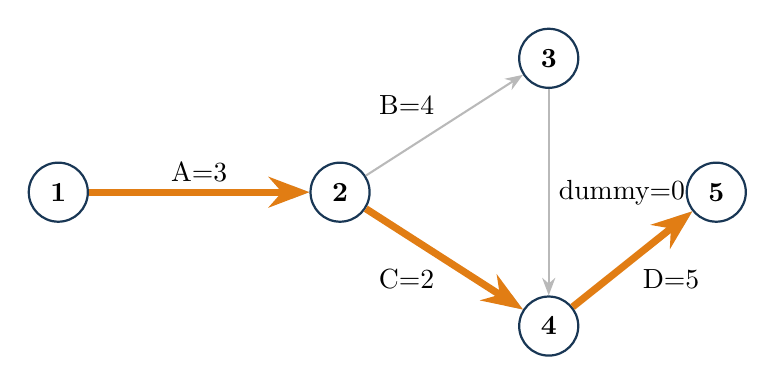
\begin{tikzpicture}[node distance=2.8cm]
\node[event](1){1};\node[event,right=of 1](2){2};\node[event,above right=1.15cm and 2.1cm of 2](3){3};\node[event,below right=1.15cm and 2.1cm of 2](4){4};\node[event,right=4.0cm of 2](5){5};
\draw[basepath](1)--node[above]{A=3}(2);\draw[basepath](2)--node[above left]{B=4}(3);\draw[basepath](2)--node[below left]{C=2}(4);\draw[basepath](3)--node[right]{dummy=0}(4);\draw[basepath](4)--node[below right]{D=5}(5);
\draw[highlightpath](1)--(2);\draw[highlightpath](2)--(4);\draw[highlightpath](4)--(5);
\end{tikzpicture}
\vspace{0.08cm}
\par\textbf{Step 1:} Selected path is $A\!\to\!C\!\to\!D$.
\par\textbf{Step 2:} Add the activity durations.
\[
P_2=3+2+5=10\text{ days}
\]
\pause
\textbf{Path 2 duration: }\boxed{10\text{ days}}
\end{frame}

\begin{frame}{Path Comparison and Project Duration}
\begin{align*}
P_1&=A+B+D=3+4+5=12\text{ days},\\
P_2&=A+C+D=3+2+5=10\text{ days}.
\end{align*}
\pause
\[
T_{project}=\max(12,10)=\boxed{12\text{ days}}
\]
\criticaltext{Therefore, the longest-duration path controls the project duration.}
\end{frame}

% =========================================================
% PERT
% =========================================================
\section{PERT}

\begin{frame}{PERT: What?}
\textbf{PERT = Programme Evaluation and Review Technique.}
\begin{block}{Purpose}
PERT is used when activity durations are uncertain.
\end{block}
\begin{itemize}
  \item Each activity is represented by three time estimates.
  \item The estimates are combined into an expected time and a measure of uncertainty.
\end{itemize}
\end{frame}

\begin{frame}{PERT: Why Three Time Estimates?}
\begin{itemize}
  \item A single deterministic duration may not represent uncertainty adequately.
  \item $a$ represents favourable conditions.
  \item $m$ represents the most likely duration.
  \item $b$ represents unfavourable conditions.
  \item PERT combines these estimates into expected time and uncertainty.
\end{itemize}
\end{frame}

\begin{frame}{PERT: Three Time Estimates}
\begin{description}
\item[$a$] Optimistic time — minimum/favourable estimate.
\item[$m$] Most likely time — normal expected duration.
\item[$b$] Pessimistic time — maximum reasonable estimate.
\end{description}
\end{frame}

\begin{frame}{PERT Expected Activity Time}
\[
\boxed{t_e=\frac{a+4m+b}{6}}
\]
\begin{itemize}
  \item The most-likely estimate receives four times the weight of each extreme estimate.
  \item The result is a weighted average used as the activity's expected duration.
\end{itemize}
\end{frame}

\begin{frame}{PERT Variance and Standard Deviation}
\[
\boxed{\sigma^2=\left(\frac{b-a}{6}\right)^2}
\]
\[
\boxed{\sigma=\frac{b-a}{6}}
\]
\vspace{0.2cm}
Larger separation between $a$ and $b$ means greater estimated uncertainty.
\end{frame}

\begin{frame}{PERT Numerical Example: Expected Time and Variance}
Given:
\[
a=2,\qquad m=5,\qquad b=8
\]
\pause
\[t_e=\frac{a+4m+b}{6}\]
\pause
\[t_e=\frac{2+4(5)+8}{6}\]
\pause
\[t_e=\frac{30}{6}=\boxed{5}\]
\pause
\[\sigma^2=\left(\frac{b-a}{6}\right)^2\]
\pause
\[\sigma^2=\left(\frac{8-2}{6}\right)^2=\boxed{1}\]
\end{frame}

\begin{frame}{PERT Activity Table: Example}
\centering
\begin{tabular}{c|ccc|cc}
\toprule
Act. & $a$ & $m$ & $b$ & $t_e$ & $\sigma^2$\\
\midrule
A & 2 & 4 & 8 & 4.00 & 1.00\\
B & 1 & 2 & 3 & 2.00 & 0.11\\
C & 3 & 5 & 7 & 5.00 & 0.44\\
\bottomrule
\end{tabular}
\vspace{0.3cm}

Each uncertain activity is converted to an expected duration and variance.
\end{frame}

\begin{frame}{PERT Project Expected Duration}
\begin{enumerate}
  \item Identify the path controlling project completion using expected activity times.
  \item Add the expected times of activities on that path:
\end{enumerate}
\[
\boxed{\mu=\sum_{\text{critical path}}t_e}
\]
\end{frame}

\begin{frame}{PERT Project Variance and Standard Deviation}
For the selected critical path:
\[
\boxed{\sigma_p^2=\sum_{\text{critical path}}\sigma_i^2}
\]
\[
\boxed{\sigma_p=\sqrt{\sum_{\text{critical path}}\sigma_i^2}}
\]
\end{frame}

\begin{frame}{PERT: Assumptions for Basic Syllabus Problems}
\begin{itemize}
  \item Activity-time uncertainty is represented by $a$, $m$ and $b$.
  \item Expected activity times are used for basic network scheduling.
  \item Critical-path activity variances are combined for the project variance approximation.
  \item Project completion time is approximated using a normal distribution for probability calculations.
\end{itemize}
\end{frame}

% =========================================================
% CPM
% =========================================================
\section{CPM and Critical Path}

\begin{frame}{CPM: What?}
\textbf{CPM = Critical Path Method.}
\begin{block}{Purpose}
CPM is a network scheduling technique in which activity durations are treated as known/deterministic for the basic calculation.
\end{block}
\end{frame}

\begin{frame}{CPM: Why?}
\begin{itemize}
  \item Determine project completion time.
  \item Identify activities controlling completion.
  \item Calculate float/scheduling flexibility.
  \item Provide the basis for project cost analysis and crashing.
\end{itemize}
\end{frame}

\begin{frame}{PERT and CPM: Basic Distinction}
\centering
\small
\begin{tabular}{l|c|c}
\toprule
 & PERT & CPM\\
\midrule
Activity time & Uncertain & Known/deterministic\\
Basic estimate & $a,m,b$ & Single duration\\
Main emphasis & Time uncertainty & Critical path / time-cost decisions\\
Probability & Included & Not inherent to basic CPM\\
\bottomrule
\end{tabular}
\end{frame}

\begin{frame}{CPM Worked Example: Activity Data}
\centering\small
\begin{tabular}{c|c|c}
\toprule
Activity & Duration & Immediate predecessor(s)\\
\midrule
A & 4 & --\\
B & 3 & A\\
C & 5 & A\\
D & 2 & B\\
E & 4 & B\\
F & 3 & C\\
G & 2 & D, F\\
H & 5 & E, G\\
I & 3 & H\\
\bottomrule
\end{tabular}
\vspace{0.3cm}
\begin{itemize}
  \item Find all complete paths, project duration, ES/EF, LS/LF, float and critical path.
  \item $G$ starts only after both $D$ and $F$ finish; $H$ starts only after both $E$ and $G$ finish.
\end{itemize}
\end{frame}

\begin{frame}{CPM Worked Network}
\centering
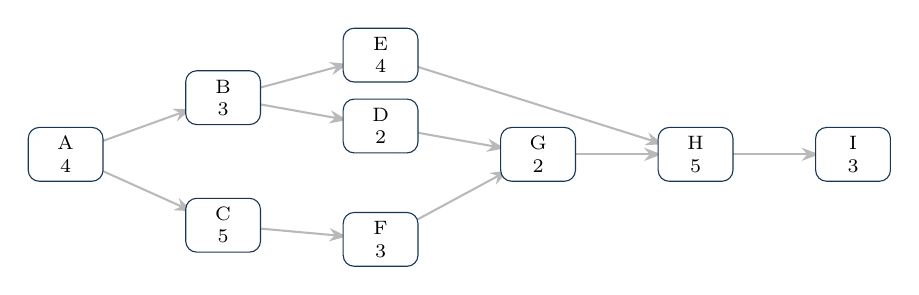
\begin{tikzpicture}[x=1cm,y=0.9cm]\coordinate (A) at (0,0);
\coordinate (B) at (2,0.8);
\coordinate (C) at (2,-1);
\coordinate (D) at (4,0.4);
\coordinate (E) at (4,1.4);
\coordinate (F) at (4,-1.2);
\coordinate (G) at (6,0);
\coordinate (H) at (8,0);
\coordinate (I) at (10,0);









\draw[actpath](A)--(B);\draw[actpath](A)--(C);\draw[actpath](B)--(D);\draw[actpath](B)--(E);\draw[actpath](C)--(F);\draw[actpath](D)--(G);\draw[actpath](F)--(G);\draw[actpath](E)--(H);\draw[actpath](G)--(H);\draw[actpath](H)--(I);

\node[act] at (0,0) {A\\4};
\node[act] at (2,0.8) {B\\3};
\node[act] at (2,-1) {C\\5};
\node[act] at (4,0.4) {D\\2};
\node[act] at (4,1.4) {E\\4};
\node[act] at (4,-1.2) {F\\3};
\node[act] at (6,0) {G\\2};
\node[act] at (8,0) {H\\5};
\node[act] at (10,0) {I\\3};
\end{tikzpicture}
\vspace{0.2cm}
\begin{itemize}
  \item $G$ waits for both $D$ and $F$.
  \item $H$ waits for both $E$ and $G$.
\end{itemize}
\end{frame}

\begin{frame}{Path 1 Highlighted: $A-B-D-G-H-I$}
\centering
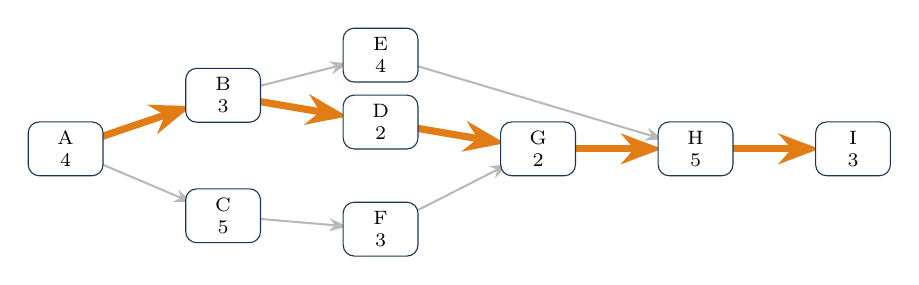
\begin{tikzpicture}[x=1cm,y=0.85cm]\coordinate (A) at (0,0);
\coordinate (B) at (2,0.8);
\coordinate (C) at (2,-1);
\coordinate (D) at (4,0.4);
\coordinate (E) at (4,1.4);
\coordinate (F) at (4,-1.2);
\coordinate (G) at (6,0);
\coordinate (H) at (8,0);
\coordinate (I) at (10,0);

\draw[actpath](A)--(B);\draw[actpath](A)--(C);\draw[actpath](B)--(D);\draw[actpath](B)--(E);\draw[actpath](C)--(F);\draw[actpath](D)--(G);\draw[actpath](F)--(G);\draw[actpath](E)--(H);\draw[actpath](G)--(H);\draw[actpath](H)--(I);
\draw[acthighlight](A)--(B);\draw[acthighlight](B)--(D);\draw[acthighlight](D)--(G);\draw[acthighlight](G)--(H);\draw[acthighlight](H)--(I);

\node[act] at (0,0) {A\\4};
\node[act] at (2,0.8) {B\\3};
\node[act] at (2,-1) {C\\5};
\node[act] at (4,0.4) {D\\2};
\node[act] at (4,1.4) {E\\4};
\node[act] at (4,-1.2) {F\\3};
\node[act] at (6,0) {G\\2};
\node[act] at (8,0) {H\\5};
\node[act] at (10,0) {I\\3};
\end{tikzpicture}
\vspace{0.08cm}
\par\textbf{Step 1:} Selected path is $A-B-D-G-H-I$.
\pause
\par\textbf{Step 2:} Add durations.
\[
P_1=4+3+2+2+5+3=19\text{ days}
\]
\pause
\textbf{Path 1 duration: }\boxed{19\text{ days}}
\end{frame}

\begin{frame}{Path 2 Highlighted: $A-C-F-G-H-I$}
\centering
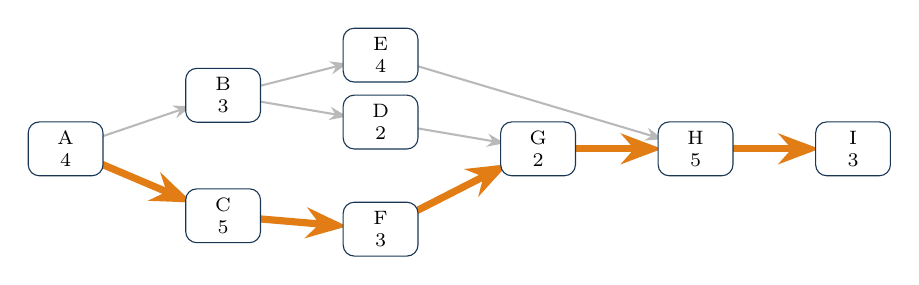
\begin{tikzpicture}[x=1cm,y=0.85cm]\coordinate (A) at (0,0);
\coordinate (B) at (2,0.8);
\coordinate (C) at (2,-1);
\coordinate (D) at (4,0.4);
\coordinate (E) at (4,1.4);
\coordinate (F) at (4,-1.2);
\coordinate (G) at (6,0);
\coordinate (H) at (8,0);
\coordinate (I) at (10,0);

\draw[actpath](A)--(B);\draw[actpath](A)--(C);\draw[actpath](B)--(D);\draw[actpath](B)--(E);\draw[actpath](C)--(F);\draw[actpath](D)--(G);\draw[actpath](F)--(G);\draw[actpath](E)--(H);\draw[actpath](G)--(H);\draw[actpath](H)--(I);
\draw[acthighlight](A)--(C);\draw[acthighlight](C)--(F);\draw[acthighlight](F)--(G);\draw[acthighlight](G)--(H);\draw[acthighlight](H)--(I);

\node[act] at (0,0) {A\\4};
\node[act] at (2,0.8) {B\\3};
\node[act] at (2,-1) {C\\5};
\node[act] at (4,0.4) {D\\2};
\node[act] at (4,1.4) {E\\4};
\node[act] at (4,-1.2) {F\\3};
\node[act] at (6,0) {G\\2};
\node[act] at (8,0) {H\\5};
\node[act] at (10,0) {I\\3};
\end{tikzpicture}
\vspace{0.08cm}
\par\textbf{Step 1:} Selected path is $A-C-F-G-H-I$.
\pause
\par\textbf{Step 2:} Add durations.
\[
P_2=4+5+3+2+5+3=22\text{ days}
\]
\pause
\textbf{Path 2 duration: }\boxed{22\text{ days}}
\end{frame}

\begin{frame}{Path 3 Highlighted: $A-B-E-H-I$}
\centering
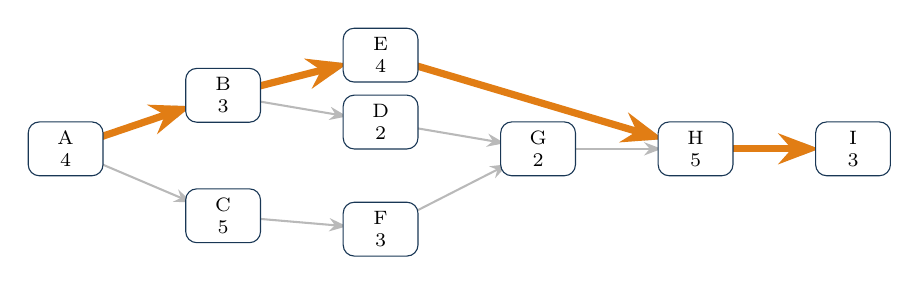
\begin{tikzpicture}[x=1cm,y=0.85cm]\coordinate (A) at (0,0);
\coordinate (B) at (2,0.8);
\coordinate (C) at (2,-1);
\coordinate (D) at (4,0.4);
\coordinate (E) at (4,1.4);
\coordinate (F) at (4,-1.2);
\coordinate (G) at (6,0);
\coordinate (H) at (8,0);
\coordinate (I) at (10,0);

\draw[actpath](A)--(B);\draw[actpath](A)--(C);\draw[actpath](B)--(D);\draw[actpath](B)--(E);\draw[actpath](C)--(F);\draw[actpath](D)--(G);\draw[actpath](F)--(G);\draw[actpath](E)--(H);\draw[actpath](G)--(H);\draw[actpath](H)--(I);
\draw[acthighlight](A)--(B);\draw[acthighlight](B)--(E);\draw[acthighlight](E)--(H);\draw[acthighlight](H)--(I);

\node[act] at (0,0) {A\\4};
\node[act] at (2,0.8) {B\\3};
\node[act] at (2,-1) {C\\5};
\node[act] at (4,0.4) {D\\2};
\node[act] at (4,1.4) {E\\4};
\node[act] at (4,-1.2) {F\\3};
\node[act] at (6,0) {G\\2};
\node[act] at (8,0) {H\\5};
\node[act] at (10,0) {I\\3};
\end{tikzpicture}
\vspace{0.08cm}
\par\textbf{Step 1:} Selected path is $A-B-E-H-I$.
\pause
\par\textbf{Step 2:} Add durations.
\[
P_3=4+3+4+5+3=19\text{ days}
\]
\pause
\textbf{Path 3 duration: }\boxed{19\text{ days}}
\end{frame}

\begin{frame}{Path Comparison and Project Duration}
\small
\textbf{Complete paths:}
\pause
\[P_1=19\text{ days}\]
\pause
\[P_2=22\text{ days}\]
\pause
\[P_3=19\text{ days}\]
\pause
\[T_p=\max(19,22,19)=\boxed{22\text{ days}}\]
\pause
\maxmark{Maximum path duration = 22 days}
\end{frame}

\begin{frame}{Forward Pass: Meaning and Rule}
\[\boxed{EF=ES+t}\]
\pause
At a merge:
\[\boxed{ES=\max(EF_1,EF_2,\ldots)}\]
\pause
\maxmark{Forward pass uses MAXIMUM at a merge.}
\end{frame}





\begin{frame}{Forward Pass: Worked Calculation -- Part 1}

\begin{columns}[T,onlytextwidth]
\column{0.34\textwidth}
\centering
\scriptsize
\begin{tabular}{c|c|c}
\toprule
Act. & $t$ & Pred.\\\midrule
A&4&--\\
B&3&A\\
C&5&A\\
D&2&B\\
E&4&B\\
F&3&C\\
\bottomrule
\end{tabular}
\vspace{0.2cm}
\begin{block}{Rule}
\centering $EF=ES+t$
\end{block}

\column{0.62\textwidth}
\teachstep{Step 1 -- Activity A}
\[
ES_A=0,\qquad EF_A=0+4=\boxed{4}
\]
\pause
\teachstep{Step 2 -- Activity B}
\[
ES_B=4,\qquad EF_B=4+3=\boxed{7}
\]
\pause
\teachstep{Step 3 -- Activity C}
\[
ES_C=4,\qquad EF_C=4+5=\boxed{9}
\]
\end{columns}

\end{frame}

\begin{frame}{Forward Pass: Worked Calculation -- Part 2}

\begin{columns}[T,onlytextwidth]
\column{0.32\textwidth}
\centering\scriptsize
\begin{tabular}{c|c|c}\toprule
Act.&$t$&Pred.\\\midrule
D&2&B\\ E&4&B\\ F&3&C\\\bottomrule
\end{tabular}
\vspace{0.12cm}
\begin{block}{Direct successor}
\centering $ES=EF_{\rm pred}$
\end{block}
\column{0.64\textwidth}
\footnotesize
\setlength{\abovedisplayskip}{2pt}\setlength{\belowdisplayskip}{2pt}
\teachstep{Step 4 -- Activity D}
\[
ES_D=EF_B=7,\quad EF_D=7+2=\boxed{9}
\]
\pause
\teachstep{Step 5 -- Activity E}
\[
ES_E=EF_B=7,\quad EF_E=7+4=\boxed{11}
\]
\pause
\teachstep{Step 6 -- Activity F}
\[
ES_F=EF_C=9,\quad EF_F=9+3=\boxed{12}
\]
\end{columns}

\end{frame}

\begin{frame}{Forward Pass: Worked Calculation -- Part 3}

\begin{columns}[T,onlytextwidth]
\column{0.32\textwidth}
\centering\scriptsize
\begin{tabular}{c|c|c}
\toprule
Activity & Duration & Predecessor(s)\\
\midrule
G & 2 & D, F\\
H & 5 & E, G\\
I & 3 & H\\
\bottomrule
\end{tabular}
\vspace{0.12cm}
\begin{block}{Merge rule}
\centering $ES=\max(EF_1,EF_2,\ldots)$
\end{block}
\column{0.64\textwidth}
\footnotesize
\setlength{\abovedisplayskip}{2pt}\setlength{\belowdisplayskip}{2pt}
\teachstep{Step 7 -- Activity G: two predecessors}
\[
ES_G=\max(9,12)=\boxed{12}
\]
\pause
\teachstep{Step 8 -- Activity G}
\[
EF_G=12+2=\boxed{14}
\]
\pause
\teachstep{Step 9 -- Activity H: two predecessors}
\[
ES_H=\max(11,14)=\boxed{14}
\]
\end{columns}

\end{frame}

\begin{frame}{Forward Pass: Worked Calculation -- Part 4}
\begin{columns}[T,onlytextwidth]
\column{0.32\textwidth}
\centering\scriptsize
\begin{tabular}{c|c|c}
\toprule
Activity & Duration & Predecessor(s)\\
\midrule
H & 5 & E, G\\
I & 3 & H\\
\bottomrule
\end{tabular}
\vspace{0.12cm}
\begin{block}{Project finish}
\centering $T_p=EF_I$
\end{block}
\column{0.64\textwidth}
\footnotesize
\setlength{\abovedisplayskip}{2pt}\setlength{\belowdisplayskip}{2pt}
\teachstep{Step 10 -- Activity H}
\[
EF_H=14+5=\boxed{19}
\]
\pause
\teachstep{Step 11 -- Activity I}
\[
ES_I=19,\quad EF_I=19+3=\boxed{22}
\]
\pause
\maxmark{Project duration from the forward pass = 22 days}
\end{columns}
\end{frame}

\begin{frame}{Forward Pass: Complete Table}
\centering\small
\begin{tabular}{c|c|c|c}
\toprule Activity & $t$ & ES & EF\\\midrule
A&4&0&4\\B&3&4&7\\C&5&4&9\\D&2&7&9\\E&4&7&11\\F&3&9&12\\G&2&12&14\\H&5&14&19\\I&3&19&22\\\bottomrule
\end{tabular}
\vspace{0.25cm}
\maxmark{Forward pass complete: 22 days}
\end{frame}

\begin{frame}{Backward Pass: Meaning and Rule}
\[\boxed{LS=LF-t}\]
\pause
At a split:
\[\boxed{LF=\min(LS_1,LS_2,\ldots)}\]
\pause
\minmark{Backward pass uses MINIMUM at a split.}
\end{frame}





\begin{frame}{Backward Pass: Worked Calculation -- Part 1}

\begin{columns}[T,onlytextwidth]
\column{0.34\textwidth}
\centering
\scriptsize
\begin{tabular}{c|c|c}
\toprule
Act. & $t$ & Successor\\\midrule
I&3&--\\
H&5&I\\
G&2&H\\
E&4&H\\
D&2&G\\
F&3&G\\
\bottomrule
\end{tabular}
\vspace{0.2cm}
\begin{block}{Rule}
\centering $LS=LF-t$
\end{block}

\column{0.62\textwidth}
\teachstep{Step 1 -- Activity I}
\[
LF_I=22,\qquad LS_I=22-3=\boxed{19}
\]
\pause
\teachstep{Step 2 -- Activity H}
\[
LF_H=LS_I=19,\qquad LS_H=19-5=\boxed{14}
\]
\pause
\teachstep{Step 3 -- Activity G}
\[
LF_G=LS_H=14,\qquad LS_G=14-2=\boxed{12}
\]
\end{columns}

\end{frame}

\begin{frame}{Backward Pass: Worked Calculation -- Part 2}

\begin{columns}[T,onlytextwidth]
\column{0.32\textwidth}
\centering\scriptsize
\begin{tabular}{c|c|c}\toprule
Act.&$t$&Succ.\\\midrule
E&4&H\\ D&2&G\\ F&3&G\\\bottomrule
\end{tabular}
\vspace{0.12cm}
\begin{block}{Direct successor}
\centering $LF=LS_{\rm succ}$
\end{block}
\column{0.64\textwidth}
\footnotesize
\setlength{\abovedisplayskip}{2pt}\setlength{\belowdisplayskip}{2pt}
\teachstep{Step 4 -- Activity E}
\[
LF_E=14,\quad LS_E=14-4=\boxed{10}
\]
\pause
\teachstep{Step 5 -- Activity D}
\[
LF_D=12,\quad LS_D=12-2=\boxed{10}
\]
\pause
\teachstep{Step 6 -- Activity F}
\[
LF_F=12,\quad LS_F=12-3=\boxed{9}
\]
\end{columns}

\end{frame}

\begin{frame}{Backward Pass: Worked Calculation -- Part 3}

\begin{columns}[T,onlytextwidth]
\column{0.32\textwidth}
\centering\scriptsize
\begin{tabular}{c|c|c}\toprule
Act.&$t$&Succ.\\\midrule
B&3&D,E\\ C&5&F\\\bottomrule
\end{tabular}
\vspace{0.12cm}
\begin{block}{Split rule}
\centering $LF=\min(LS_1,LS_2,\ldots)$
\end{block}
\column{0.64\textwidth}
\footnotesize
\setlength{\abovedisplayskip}{2pt}\setlength{\belowdisplayskip}{2pt}
\teachstep{Step 7 -- Activity B: two successors}
\[
LF_B=\min(10,10)=\boxed{10}
\]
\pause
\teachstep{Step 8 -- Activity B}
\[
LS_B=10-3=\boxed{7}
\]
\pause
\teachstep{Step 9 -- Activity C}
\[
LF_C=9,\quad LS_C=9-5=\boxed{4}
\]
\end{columns}

\end{frame}

\begin{frame}{Backward Pass: Worked Calculation -- Part 4}
\begin{columns}[T,onlytextwidth]
\column{0.32\textwidth}
\centering\scriptsize
\begin{tabular}{c|c|c}\toprule
Act.&$t$&Succ.\\\midrule
A&4&B,C\\\bottomrule
\end{tabular}
\vspace{0.12cm}
\begin{block}{Project start}
\centering $LS_A=0$
\end{block}
\column{0.64\textwidth}
\footnotesize
\setlength{\abovedisplayskip}{2pt}\setlength{\belowdisplayskip}{2pt}
\teachstep{Step 10 -- Activity A: two successors}
\[
LF_A=\min(7,4)=\boxed{4}
\]
\pause
\teachstep{Step 11 -- Activity A}
\[
LS_A=4-4=\boxed{0}
\]
\pause
\minmark{Backward pass complete: minimum successor values control each split.}
\end{columns}
\end{frame}

\begin{frame}{Backward Pass: Complete Table}
\centering\small
\begin{tabular}{c|c|c|c}
\toprule Activity & $t$ & LS & LF\\\midrule
A&4&0&4\\B&3&7&10\\C&5&4&9\\D&2&10&12\\E&4&10&14\\F&3&9&12\\G&2&12&14\\H&5&14&19\\I&3&19&22\\\bottomrule
\end{tabular}
\end{frame}

\begin{frame}{Total Float: Meaning and Formula}
\[\boxed{TF=LS-ES=LF-EF}\]
\pause
$TF=0$ means no scheduling flexibility in the basic CPM calculation.
\pause
$TF>0$ means positive scheduling flexibility.
\end{frame}

\begin{frame}{Total Float: Complete Calculation}
\small
\[
\boxed{TF=LS-ES=LF-EF}
\]
\begin{center}
\begin{tabular}{c|c|c|c|c}
\toprule Activity & ES & LS & TF & Interpretation\\\midrule
A&0&0&0&Critical\\B&4&7&3&Float\\C&4&4&0&Critical\\D&7&10&3&Float\\E&7&10&3&Float\\F&9&9&0&Critical\\G&12&12&0&Critical\\H&14&14&0&Critical\\I&19&19&0&Critical\\\bottomrule
\end{tabular}
\end{center}
\pause
\begin{center}\parbox{0.82\textwidth}{\centering Zero-float activities are the activities on the critical path for this network.}\end{center}
\end{frame}

\begin{frame}{Identifying the Critical Path}
\small
\textbf{Compare the complete paths with the float calculation.}
\pause
\[A-B-D-G-H-I=19\text{ days}\]
\pause
\[A-C-F-G-H-I=22\text{ days}\]
\pause
\[A-B-E-H-I=19\text{ days}\]
\pause
\[T_p=\max(19,22,19)=\boxed{22\text{ days}}\]
\pause
\criticaltext{Critical Path = A--C--F--G--H--I}
\end{frame}

\begin{frame}{Critical Path Highlighted}
\centering
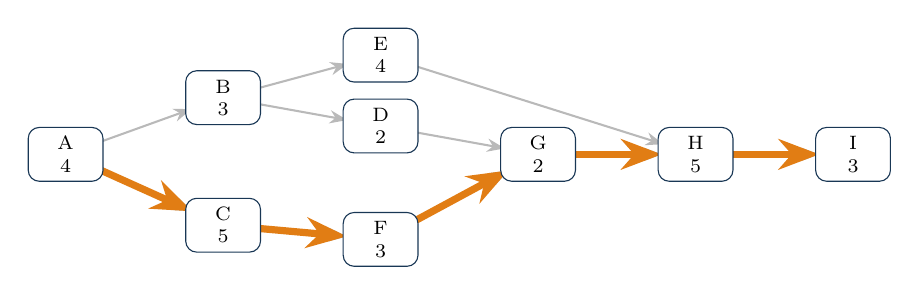
\begin{tikzpicture}[x=1cm,y=0.9cm]\coordinate (A) at (0,0);
\coordinate (B) at (2,0.8);
\coordinate (C) at (2,-1);
\coordinate (D) at (4,0.4);
\coordinate (E) at (4,1.4);
\coordinate (F) at (4,-1.2);
\coordinate (G) at (6,0);
\coordinate (H) at (8,0);
\coordinate (I) at (10,0);

\draw[actpath](A)--(B);\draw[actpath](A)--(C);\draw[actpath](B)--(D);\draw[actpath](B)--(E);\draw[actpath](C)--(F);\draw[actpath](D)--(G);\draw[actpath](F)--(G);\draw[actpath](E)--(H);\draw[actpath](G)--(H);\draw[actpath](H)--(I);
\draw[acthighlight](A)--(C);\draw[acthighlight](C)--(F);\draw[acthighlight](F)--(G);\draw[acthighlight](G)--(H);\draw[acthighlight](H)--(I);

\node[act] at (0,0) {A\\4};
\node[act] at (2,0.8) {B\\3};
\node[act] at (2,-1) {C\\5};
\node[act] at (4,0.4) {D\\2};
\node[act] at (4,1.4) {E\\4};
\node[act] at (4,-1.2) {F\\3};
\node[act] at (6,0) {G\\2};
\node[act] at (8,0) {H\\5};
\node[act] at (10,0) {I\\3};
\end{tikzpicture}
\vspace{0.15cm}
\criticaltext{Critical path: A--C--F--G--H--I}
\end{frame}

\begin{frame}{PERT: Probability of Completing Within a Given Time}
For target completion time $T$:
\[
\boxed{Z=\frac{T-\mu}{\sigma_p}}
\]
where:
\begin{itemize}
  \item $\mu$ = expected project duration,
  \item $\sigma_p$ = project standard deviation.
\end{itemize}
The normal cumulative probability corresponding to $Z$ gives the approximate probability of completion by $T$.
\end{frame}

\begin{frame}{Probability: Interpretation of $Z$}
\begin{itemize}
  \item $Z=0$: target time equals expected project duration.
  \item $Z>0$: target time is later than expected; probability is above 0.5 under the approximation.
  \item $Z<0$: target time is earlier than expected; probability is below 0.5.
  \item $|Z|$ measures the distance from the expected duration in standard-deviation units.
\end{itemize}
\end{frame}

\begin{frame}{PERT Probability: Worked Problem}
Given:
\[
\mu=20\text{ days},\qquad \sigma_p=2\text{ days},\qquad T=22\text{ days}
\]
\pause
\[Z=\frac{T-\mu}{\sigma_p}\]
\pause
\[Z=\frac{22-20}{2}\]
\pause
\[\boxed{Z=1}\]
\pause
\[P(Z\le1)=0.8413\]
\pause
\answer{Probability of completion by 22 days = 84.13\%}
\end{frame}

\begin{frame}{PERT Probability: Another Interpretation}
If:
\[
T=\mu-2\sigma_p
\]
then:
\[
Z=-2
\]
\pause
\[
P(Z\le -2)\approx0.0228
\]
\answer{Approximate probability = 2.28\%}
\end{frame}

\begin{frame}{Standard Normal Table: How It Is Used}
\begin{enumerate}
  \item Calculate $Z=(T-\mu)/\sigma_p$.
  \item Locate $Z$ in the standard normal cumulative table.
  \item Read the cumulative probability.
  \item For negative $Z$, use symmetry:
  \[
  \Phi(-z)=1-\Phi(z).
  \]
\end{enumerate}
\end{frame}

\begin{frame}{Standard Normal Cumulative Values Used in Basic Problems}
\centering
\begin{tabular}{c|cccccccccc}
\toprule
$z$ & 0.0 & 0.5 & 1.0 & 1.5 & 2.0 & -0.5 & -1.0 & -1.5 & -2.0\\
\midrule
$\Phi(z)$ & .5000 & .6915 & .8413 & .9332 & .9772 & .3085 & .1587 & .0668 & .0228\\
\bottomrule
\end{tabular}
\vspace{0.3cm}

Use the full standard normal table when a problem gives a different $Z$ value.
\end{frame}

% =========================================================
% PROJECT COST ANALYSIS
% =========================================================
\section{Project Cost Analysis}

\begin{frame}{Project Cost Analysis: What?}
\begin{itemize}
  \item Project cost analysis compares project time with associated costs.
  \item For crashing, distinguish normal and crash time/cost.
  \item The objective is to understand the additional direct cost associated with reducing project duration.
\end{itemize}
\end{frame}

\begin{frame}{Normal Time, Crash Time, Normal Cost, Crash Cost}
\centering
\begin{tabular}{l|l}
\toprule
Quantity & Meaning\\
\midrule
Normal time $T_n$ & Duration under normal conditions\\
Crash time $T_c$ & Minimum practical duration considered for crashing\\
Normal cost $C_n$ & Cost corresponding to normal duration\\
Crash cost $C_c$ & Cost corresponding to crash duration\\
\bottomrule
\end{tabular}
\end{frame}

\begin{frame}{Cost Slope}
The additional cost per unit time reduction is:
\[
\boxed{\text{Cost slope}=\frac{C_c-C_n}{T_n-T_c}}
\]
\vspace{0.2cm}
It is meaningful only within the stated normal-to-crash time range.
\end{frame}

\begin{frame}{Physical Interpretation of Cost Slope}
\begin{block}{Meaning}
Cost slope is the incremental direct cost associated with reducing an activity's duration.
\end{block}
\begin{itemize}
  \item Smaller positive slope: smaller additional cost per unit time reduction.
  \item It is not the total project cost.
  \item It is a time-cost trade-off measure.
\end{itemize}
\end{frame}

\begin{frame}{Project Cost Analysis: Total Cost}
A basic project cost model is:
\[
\boxed{C_{total}=C_{direct}+C_{indirect}}
\]
\begin{itemize}
  \item Shorter duration can require additional direct crashing cost.
  \item Longer duration can increase time-related/indirect project cost.
  \item Therefore project duration and cost are linked by a time-cost trade-off.
\end{itemize}
\end{frame}

\begin{frame}{Project Cost Analysis: Time--Cost Relationship}
\centering
\begin{tikzpicture}[x=1cm,y=0.8cm]
\draw[->,thick](0,0)--(10,0) node[right]{Project duration};
\draw[->,thick](0,0)--(0,6) node[above]{Cost};
\draw[thick,Orange](1,5.2) .. controls (3,4.4) and (6,2.8) .. (9,1.8);
\node at (5,5.2) {illustrative direct-cost trend};
\end{tikzpicture}
\vspace{0.2cm}

The figure illustrates the principle only: reducing duration can require increasing direct cost.
\end{frame}

\begin{frame}{Cost Analysis: Multi-Activity Numerical Problem}
\centering\small
\begin{tabular}{c|cccc}
\toprule Activity & $T_n$ & $T_c$ & $C_n$ & $C_c$\\
\midrule
A&8&5&4000&5200\\
B&6&4&3000&4200\\
C&7&5&3500&4300\\
D&5&3&2500&3300\\
\bottomrule
\end{tabular}
\vspace{0.25cm}
\textbf{Required:} calculate the cost slope of each activity and compare the additional cost per unit time reduction.
\end{frame}

\begin{frame}{Cost Analysis: Step 1 -- Activity A}
\[S_A=\frac{C_c-C_n}{T_n-T_c}\]
\pause
\[S_A=\frac{5200-4000}{8-5}\]
\pause
\[S_A=\frac{1200}{3}\]
\pause
\[\boxed{S_A=400\text{ per time unit}}\]
\end{frame}

\begin{frame}{Cost Analysis: Step 2 -- Activities B and C}
\small
\par\textbf{Step 1 -- Activity B}
\[
S_B=\frac{4200-3000}{6-4}=\boxed{600}
\]
\pause
\par\textbf{Step 2 -- Activity C}
\[
S_C=\frac{4300-3500}{7-5}=\boxed{400}
\]
\end{frame}

\begin{frame}{Cost Analysis: Step 3 -- Activity D and Comparison}
\small
\par\textbf{Step 1 -- Activity D}
\[
S_D=\frac{3300-2500}{5-3}=\boxed{400}
\]
\pause
\par\textbf{Step 2: Compare all slopes.}
\begin{center}
\begin{tabular}{c|c}\toprule Activity & Cost slope\\\midrule A&400\\B&600\\C&400\\D&400\\\bottomrule\end{tabular}
\end{center}
\pause
\textbf{Interpretation:} a lower feasible slope means a smaller additional direct cost for one unit of reduction.
\end{frame}

% =========================================================
% PROJECT CRASHING
% =========================================================
\section{Project Crashing}

\begin{frame}{Project Crashing: What?}
\begin{block}{Definition}
Crashing means shortening project duration by reducing the duration of selected activities, normally with additional direct cost.
\end{block}
\begin{itemize}
  \item Only crashable activities can be shortened.
  \item Crashing a noncritical activity may not reduce project duration.
  \item Critical-path identification is therefore essential before crashing.
\end{itemize}
\end{frame}

\begin{frame}{Project Crashing: When and Why?}
\textbf{When?}
\begin{itemize}
  \item When required completion time is shorter than the current schedule.
\end{itemize}
\textbf{Why?}
\begin{itemize}
  \item To achieve a shorter completion time subject to additional cost.
  \item To study the time-cost trade-off for simple project decisions.
\end{itemize}
\end{frame}

\begin{frame}{Project Crashing: Procedure}
\begin{enumerate}
  \item Construct the CPM network and find the current critical path.
  \item Identify crashable activities on the current critical path.
  \item Calculate cost slopes.
  \item Select an appropriate crashable critical activity.
  \item Reduce its duration within its crash limit.
  \item Recalculate the network and critical path.
  \item Repeat until the required duration is reached or no further feasible crashing is possible.
\end{enumerate}
\end{frame}

\begin{frame}{Crashing: Simple Decision Rule}
For a required one-unit reduction, compare the cost slopes of crashable critical activities.
\[
\boxed{\text{Choose the feasible critical activity with the lower cost slope}}
\]
subject to its available crash range and the current network logic.
\end{frame}

\begin{frame}{Crashing: Multi-Step Worked Problem}
\centering\small
\begin{tabular}{c|cccc|c}
\toprule Activity & $T_n$ & $T_c$ & $C_n$ & $C_c$ & Slope\\
\midrule
A&6&4&600&800&100\\
B&5&3&900&1200&150\\
C&7&5&700&1100&200\\
D&4&2&500&800&150\\
\bottomrule
\end{tabular}
\vfill
\begin{beamercolorbox}[wd=0.90\textwidth,sep=0.16cm,center]{normal text}
\small Suppose the current critical path contains A and B; a two-unit project reduction is required.
\end{beamercolorbox}
\end{frame}

\begin{frame}{Crashing: Step 1 -- Select the First Activity}
\small
\par\textbf{Step 1:} Identify crashable activities on the current critical path.
A and B are crashable critical activities.
\pause
\par\textbf{Step 2:} Compare their cost slopes.
\[
S_A=100,\qquad S_B=150
\]
\pause
\par\textbf{Step 3:} Select A because its slope is lower.
\[
T_A:6\rightarrow5,\qquad C_A:600\rightarrow700
\]
\end{frame}

\begin{frame}{Crashing: Step 2 -- Recalculate the Network}
\small
\par\textbf{Step 1:} Recalculate the affected path duration.
\pause
\par\textbf{Step 2:} Compare the new duration with the other complete paths.
\pause
\par\textbf{Step 3:} Check whether the same path remains critical.
\pause
\par\textbf{Step 4:} Confirm that one more unit of project reduction is still required.
\textbf{Rule:} every crash decision must be followed by a network recheck.
\end{frame}

\begin{frame}{Crashing: Step 3 -- Second Reduction}
\small
\par\textbf{Step 1:} If A cannot be reduced further, examine the remaining critical activities.
\pause
\par\textbf{Step 2:} Activity B has:
\[
S_B=\boxed{150\text{ per time unit}}
\]
\pause
\par\textbf{Step 3:} Reduce B by one unit within its crash limit.
\[
T_B:5\rightarrow4,\qquad C_B:900\rightarrow1050
\]
\end{frame}

\begin{frame}{Crashing: Step 4 -- Additional Cost}
\small
\par\textbf{Step 1:} Cost of the first one-unit reduction on A.
\[
\Delta C_A=1(100)=\boxed{100}
\]
\pause
\par\textbf{Step 2:} Cost of the second one-unit reduction on B.
\[
\Delta C_B=1(150)=\boxed{150}
\]
\pause
\par\textbf{Step 3:} Total additional direct cost.
\[
\Delta C=100+150=\boxed{250}
\]
\end{frame}

\begin{frame}{Crashing: Final Check}
\textbf{Do not stop at the cost calculation.}
\pause
\begin{enumerate}
  \item Recalculate all complete path durations.
  \pause
  \item Re-identify the critical path.
  \pause
  \item Confirm the required project reduction.
  \pause
  \item Check that no further crash limit or network constraint has been violated.
\end{enumerate}
\pause
\criticaltext{A crashing solution is valid only after the network is rechecked.}
\end{frame}

\begin{frame}{Crashing: Why the Critical Path Must Be Rechecked}
After crashing an activity:
\begin{enumerate}
  \item Recalculate affected path durations.
  \item Check whether another path has become equally long or longer.
  \item Re-identify the critical path.
\end{enumerate}
\vspace{0.2cm}
\criticaltext{The critical path can change after crashing.}
\end{frame}

\begin{frame}{Crashing: Simple Path Illustration}
Suppose:
\[
P_1=12\text{ days},\qquad P_2=9\text{ days}
\]
\pause
After one-day reduction on a critical activity of $P_1$:
\[
P_1=11,\qquad P_2=9,\qquad T_p=\boxed{11\text{ days}}
\]
\end{frame}

\begin{frame}{Crashing: When Two Paths Become Critical}
Suppose:
\[
P_1=10,\qquad P_2=10
\]
\pause
\[
T_p=\boxed{10\text{ days}}
\]
Both paths have the same maximum duration.
\criticaltext{Therefore, both paths are critical in this state.}
\end{frame}

% =========================================================
% INTEGRATED NUMERICALS
% =========================================================
\section{Worked Problems}

\begin{frame}{Integrated PERT Problem: Data}
\centering
\begin{tabular}{c|ccc}
\toprule
Activity & $a$ & $m$ & $b$\\
\midrule
A & 2 & 4 & 8\\
B & 1 & 2 & 3\\
C & 3 & 5 & 7\\
\bottomrule
\end{tabular}
\vspace{0.3cm}

Assume these activities form the relevant critical path for the simple probability calculation.
\end{frame}

\begin{frame}{Integrated PERT: Expected Times and Variances}
\centering
\begin{tabular}{c|ccc|cc}
\toprule
Activity & $a$ & $m$ & $b$ & $t_e$ & $\sigma^2$\\
\midrule
A & 2 & 4 & 8 & 4.00 & 1.00\\
B & 1 & 2 & 3 & 2.00 & 0.11\\
C & 3 & 5 & 7 & 5.00 & 0.44\\
\bottomrule
\end{tabular}
\pause
\[
t_e=\frac{a+4m+b}{6},\qquad \sigma^2=\left(\frac{b-a}{6}\right)^2
\]
\[
\mu=4+2+5=11\text{ days},\qquad \sigma_p^2=1+0.11+0.44=1.55\text{ day}^2
\]
\end{frame}

\begin{frame}{Integrated PERT: Project Standard Deviation and Probability}
\[
\sigma_p=\sqrt{1.55}\approx1.245\text{ days}
\]
\pause
For completion within 13 days:
\[
Z=\frac{13-11}{1.245}\approx1.61,
\qquad P(Z\le1.61)\approx0.9463.
\]
\answer{Approximate probability of completion within 13 days = 94.63\%}
\end{frame}


\begin{frame}{Integrated PERT Problem: Larger Data Set}
\centering\small
\begin{tabular}{c|ccc|c}
\toprule Activity & $a$ & $m$ & $b$ & Predecessor\\
\midrule
A&2&4&6&--\\
B&1&3&5&A\\
C&2&4&8&A\\
D&1&2&3&B\\
E&2&5&8&C\\
F&1&3&5&D,E\\
\bottomrule
\end{tabular}
\vfill
\begin{beamercolorbox}[wd=0.90\textwidth,sep=0.16cm,center]{normal text}
\small Use expected times to identify the controlling path; then calculate project variance and completion probability.
\end{beamercolorbox}
\end{frame}

\begin{frame}{PERT Network for the Worked Problem}
\centering
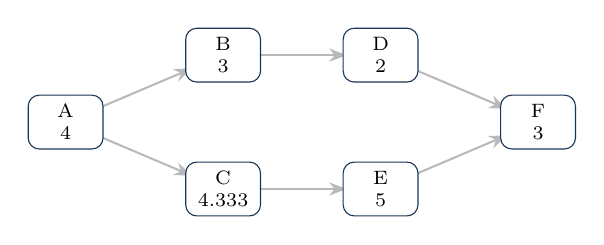
\begin{tikzpicture}[x=1cm,y=0.85cm]
\coordinate (A) at (0,0);\coordinate (B) at (2,1);\coordinate (C) at (2,-1);\coordinate (D) at (4,1);\coordinate (E) at (4,-1);\coordinate (F) at (6,0);
\draw[actpath](A)--(B);\draw[actpath](A)--(C);\draw[actpath](B)--(D);\draw[actpath](C)--(E);\draw[actpath](D)--(F);\draw[actpath](E)--(F);
\node[act] at (A) {A\\4};\node[act] at (B) {B\\3};\node[act] at (C) {C\\4.333};\node[act] at (D) {D\\2};\node[act] at (E) {E\\5};\node[act] at (F) {F\\3};
\end{tikzpicture}
\vspace{0.15cm}
The expected-time network has two complete paths to the finish.
\end{frame}

\begin{frame}{PERT Path 1 Highlighted: $A-B-D-F$}
\centering
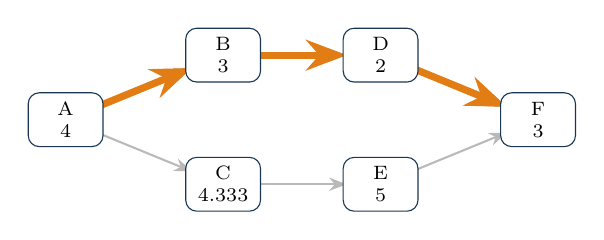
\begin{tikzpicture}[x=1cm,y=0.82cm]\coordinate (A) at (0,0);
\coordinate (B) at (2,1);
\coordinate (C) at (2,-1);
\coordinate (D) at (4,1);
\coordinate (E) at (4,-1);
\coordinate (F) at (6,0);

\draw[actpath](A)--(B);\draw[actpath](A)--(C);\draw[actpath](B)--(D);\draw[actpath](C)--(E);\draw[actpath](D)--(F);\draw[actpath](E)--(F);
\draw[acthighlight](A)--(B);\draw[acthighlight](B)--(D);\draw[acthighlight](D)--(F);

\node[act] at (0,0) {A\\4};
\node[act] at (2,1) {B\\3};
\node[act] at (2,-1) {C\\4.333};
\node[act] at (4,1) {D\\2};
\node[act] at (4,-1) {E\\5};
\node[act] at (6,0) {F\\3};
\end{tikzpicture}
\vspace{0.05cm}
\par\textbf{Step 1:} Selected path $A-B-D-F$.
\pause
\par\textbf{Step 2:} Add expected activity times.
\[
P_1=4+3+2+3=12\text{ days}
\]
\pause
\textbf{Path 1 expected duration: }\boxed{12\text{ days}}
\end{frame}

\begin{frame}{PERT Path 2 Highlighted: $A-C-E-F$}
\centering
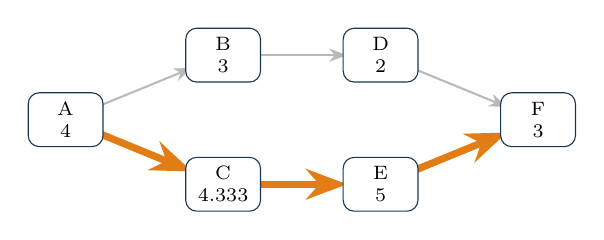
\begin{tikzpicture}[x=1cm,y=0.82cm]\coordinate (A) at (0,0);
\coordinate (B) at (2,1);
\coordinate (C) at (2,-1);
\coordinate (D) at (4,1);
\coordinate (E) at (4,-1);
\coordinate (F) at (6,0);

\draw[actpath](A)--(B);\draw[actpath](A)--(C);\draw[actpath](B)--(D);\draw[actpath](C)--(E);\draw[actpath](D)--(F);\draw[actpath](E)--(F);
\draw[acthighlight](A)--(C);\draw[acthighlight](C)--(E);\draw[acthighlight](E)--(F);

\node[act] at (0,0) {A\\4};
\node[act] at (2,1) {B\\3};
\node[act] at (2,-1) {C\\4.333};
\node[act] at (4,1) {D\\2};
\node[act] at (4,-1) {E\\5};
\node[act] at (6,0) {F\\3};
\end{tikzpicture}
\vspace{0.05cm}
\par\textbf{Step 1:} Selected path $A-C-E-F$.
\pause
\par\textbf{Step 2:} Add expected activity times.
\[
P_2=4+4.333+5+3=16.333\text{ days}
\]
\pause
\textbf{Path 2 expected duration: }\boxed{16.333\text{ days}}
\end{frame}

\begin{frame}{PERT Path Comparison}
\[P_1=12\text{ days}\]
\pause
\[P_2=16.333\text{ days}\]
\pause
\[\mu=\max(12,16.333)=\boxed{16.333\text{ days}}\]
\pause
The second path controls the expected project duration in this basic PERT calculation.
\end{frame}

\begin{frame}{Integrated PERT: Step 1 -- Activity A}
\[t_{e,A}=\frac{2+4(4)+6}{6}\]
\pause
\[t_{e,A}=\frac{24}{6}=\boxed{4}\]
\pause
\[\sigma_A^2=\left(\frac{6-2}{6}\right)^2=\boxed{0.4444}\]
\end{frame}

\begin{frame}{Integrated PERT: Step 2 -- Activities B and C}
\small
\par\textbf{Step 1 -- Activity B}
\[
t_{e,B}=\frac{1+4(3)+5}{6}=\frac{18}{6}=\boxed{3}
\]
\pause
\par\textbf{Step 2 -- Activity C}
\[
t_{e,C}=\frac{2+4(4)+8}{6}=\frac{26}{6}=\boxed{4.333}
\]
\end{frame}

\begin{frame}{Integrated PERT: Step 3 -- Activities D, E and F}
\small
\par\textbf{Step 1 -- Activity D}
\[
t_{e,D}=\frac{1+4(2)+3}{6}=\boxed{2}
\]
\pause
\par\textbf{Step 2 -- Activity E}
\[
t_{e,E}=\frac{2+4(5)+8}{6}=\boxed{5}
\]
\pause
\par\textbf{Step 3 -- Activity F}
\[
t_{e,F}=\frac{1+4(3)+5}{6}=\boxed{3}
\]
\end{frame}

\begin{frame}{Integrated PERT: Step 4 -- Compare Expected-Time Paths}
\small
\par\textbf{Step 1:} Calculate Path 1.
\[
A-B-D-F=4+3+2+3=\boxed{12\text{ days}}
\]
\pause
\par\textbf{Step 2:} Calculate Path 2.
\[
A-C-E-F=4+4.333+5+3=\boxed{16.333\text{ days}}
\]
\pause
\par\textbf{Step 3:} Select the controlling expected-time path.
\[
\mu=\max(12,16.333)=\boxed{16.333\text{ days}}
\]
\end{frame}

\begin{frame}{Integrated PERT: Step 5 -- Project Variance}
For path $A-C-E-F$:
\pause
\[\sigma_p^2=\sigma_A^2+\sigma_C^2+\sigma_E^2+\sigma_F^2\]
\pause
\[=0.4444+1.0000+1.0000+0.4444\]
\pause
\[\boxed{\sigma_p^2=2.8888}\]
\end{frame}

\begin{frame}{Integrated PERT: Step 6 -- Standard Deviation and Probability}
\small
\par\textbf{Step 1:} Calculate project standard deviation.
\[
\sigma_p=\sqrt{2.8888}=\boxed{1.700\text{ days}}
\]
\pause
\par\textbf{Step 2:} For completion within 18 days, calculate $Z$.
\[
Z=\frac{18-16.333}{1.700}=\boxed{0.98}
\]
\pause
\par\textbf{Step 3:} Read the cumulative normal probability.
\[
P(Z\le0.98)\approx\boxed{0.8365}
\]
\pause
\textbf{Probability of completion within 18 days: }\boxed{83.65\%}
\end{frame}

\begin{frame}{Integrated CPM: Complete Calculation Pattern}
\begin{enumerate}
  \item List activities and predecessors.
  \item Draw the network.
  \item List and highlight each complete path separately.
  \item Calculate each path duration.
  \item Identify the maximum path.
  \item Perform forward pass: \textbf{MAX at merges}.
  \item Perform backward pass: \textbf{MIN at splits}.
  \item Calculate float.
  \item Verify the zero-float critical path.
\end{enumerate}
\end{frame}

\begin{frame}{Integrated Cost/Crashing: Complete Pattern}
\begin{enumerate}
  \item Establish normal project duration.
  \item Identify the current critical path.
  \item Calculate cost slopes of crashable critical activities.
  \item Reduce the selected activity within its crash limit.
  \item Recalculate the network.
  \item Re-identify the critical path.
  \item Continue only if project duration is actually reduced and further crashing is feasible.
\end{enumerate}
\end{frame}

% =========================================================
% COMMON MISTAKES / FORMULAS / REVIEW
% =========================================================
\section{Review}



\begin{frame}{Formula Sheet: Job Evaluation}
\[
\boxed{J=\sum_i v_i}
\qquad\text{Factor comparison (simple additive form)}
\]
\[
\boxed{J=\sum_i p_i}
\qquad\text{Point method}
\]
Classification has no universal numerical formula; assignment is made by comparison with grade descriptions.
\end{frame}

\begin{frame}{Formula Sheet: CPM}
\[
\boxed{EF=ES+t}
\qquad
\boxed{LS=LF-t}
\]
\[
\boxed{TF=LS-ES=LF-EF}
\]
\[
\boxed{T_{project}=\text{duration of longest start-to-finish path}}
\]
\end{frame}

\begin{frame}{Formula Sheet: PERT}
\[
\boxed{t_e=\frac{a+4m+b}{6}}
\qquad
\boxed{\sigma^2=\left(\frac{b-a}{6}\right)^2}
\]
\[
\boxed{\sigma=\frac{b-a}{6}}
\qquad
\boxed{\mu=\sum_{critical\ path}t_e}
\]
\[
\boxed{\sigma_p=\sqrt{\sum_{critical\ path}\sigma_i^2}}
\qquad
\boxed{Z=\frac{T-\mu}{\sigma_p}}
\]
\end{frame}

\begin{frame}{Formula Sheet: Cost Analysis and Crashing}
\[
\boxed{C_{total}=C_{direct}+C_{indirect}}
\]
\[
\boxed{\text{Cost slope}=\frac{C_c-C_n}{T_n-T_c}}
\]
\begin{itemize}
  \item Normal condition: $T_n,C_n$.
  \item Crash condition: $T_c,C_c$.
  \item Crash only within the feasible normal-to-crash range.
  \item Recalculate the critical path after relevant crashing.
\end{itemize}
\end{frame}
\end{document}
